\documentclass[style=unh]{powerdot}
\usepackage{graphicx}

\pdsetup{
  lf={Seth Lemons (UNH)},
  rf = {An Empirical Comparison of Parallel Search Algorithms},
  list={itemsep=8pt}}


\title{An Empirical Comparison of Parallel Search Algorithms}
\author{Seth Lemons \vspace{0.2in} \\
  
\includegraphics[height=0.4in]{figures/unh-logo-words.eps} \\
  Department of Computer Science \\
  {\tt seth.lemons} at {\tt unh.edu}}
\date{\mbox{}}

\begin{document}
\maketitle

% ------------------------------------------------------------

\section[slide=false]{Introduction}

% --------------------

\begin{slide}{Goal}
  \vspace{1in}
  \begin{center}
    Evaluating parallel algorithms \\
    {\tiny Factorial and comparative analysis}
  \end{center}

\end{slide}

% --------------------

\begin{slide}{Motivation}
    \begin{center}
      What do we really know?
    \end{center}

    \begin{itemize}
    \item Lots of individual tests
    \item Not much discussion of weaknesses
    \item How do we determine parameters?
    \end{itemize}
\end{slide}

% ------------------------------------------------------------

\section{Algorithms}

% --------------------

\begin{slide}{PA*}
  \vspace{.2in}
  \begin{center}
    Parallel A*
  \end{center}

  \vspace{.1in}

  \onslide*{1}{
  \begin{itemize}[type=1]
  \item Single open and closed list
  \item Each processor grabs first node on open
  \item Lock on open list for popping best node and pushing children
  \item Lock on closed list for checking duplicates
  \end{itemize}
  }
\end{slide}

% --------------------

\begin{slide}{PRA*}
  \vspace{.2in}
  \begin{center}
    Parallel Retracting A*
  \end{center}

  \vspace{.1in}

  \onslide*{1}{
  \begin{itemize}[type=1]
  \item Hash from nodes to processors
  \item Open and closed list for each processor
  \item Each processor picks best node from its open list
  \item Children are pushed to processor which they hash to
  \item Can be made memory bounded
  \end{itemize}
  }
\end{slide}

% --------------------

\begin{slide}{KBFS}
  \vspace{.2in}
  \begin{center}
    K Best-First Search
  \end{center}

  \vspace{.1in}

  \onslide*{1}{
  \begin{itemize}[type=1]
  \item One main thread, many worker threads
  \item Main thread takes K best nodes off open list
  \item Each worker is given a node to expand
  \item Lock on open list needed for insertion only
  \item Lock on closed list for duplicate detection
  \item Main thread waits for all workers to finish before repeating
  \end{itemize}
  }
\end{slide}

% --------------------

\begin{slide}{PSDD}
  \vspace{.2in}
  \begin{center}
    Parallel Structured Duplicate Detection
  \end{center}
  \onslide*{1}{
    \begin{itemize}
    \item Abstraction function used to map states to abstract states or \emph{nblocks}
    \item For each abstract state, all successor states are known
    \item Successors of an abstract state are called its duplicate detection scope
    \end{itemize}
  }
  \onslide*{2}{
    \begin{itemize}
    \item Processors get exclusive access to a \emph{duplicate detection
      scope}
    \item Uses a breadth first search, searching all of one layer before moving on
    \end{itemize}
  }
  \onslide*{3}{
    \begin{center}
      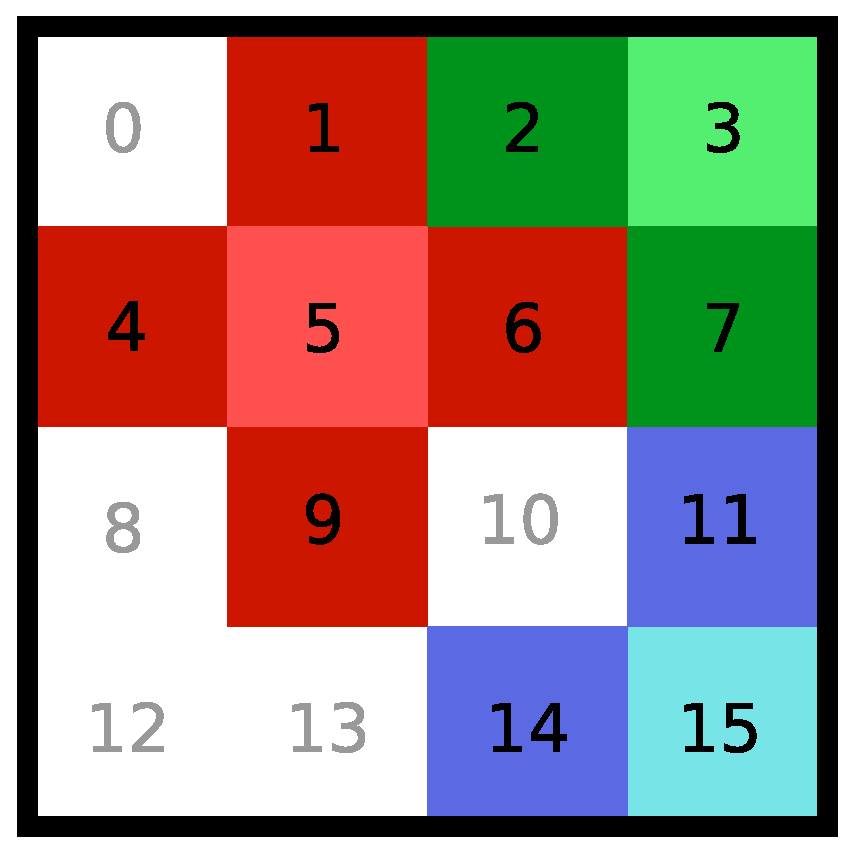
\includegraphics[width=2in]{figures/disjoint-scopes6} \\
    \end{center}

    \vspace{-.3in}
    \begin{center}
      15-Puzzle projected on the blank
    \end{center}
  }
  \onslide*{4}{
    \begin{center}
      Nblocks per thread\\
      %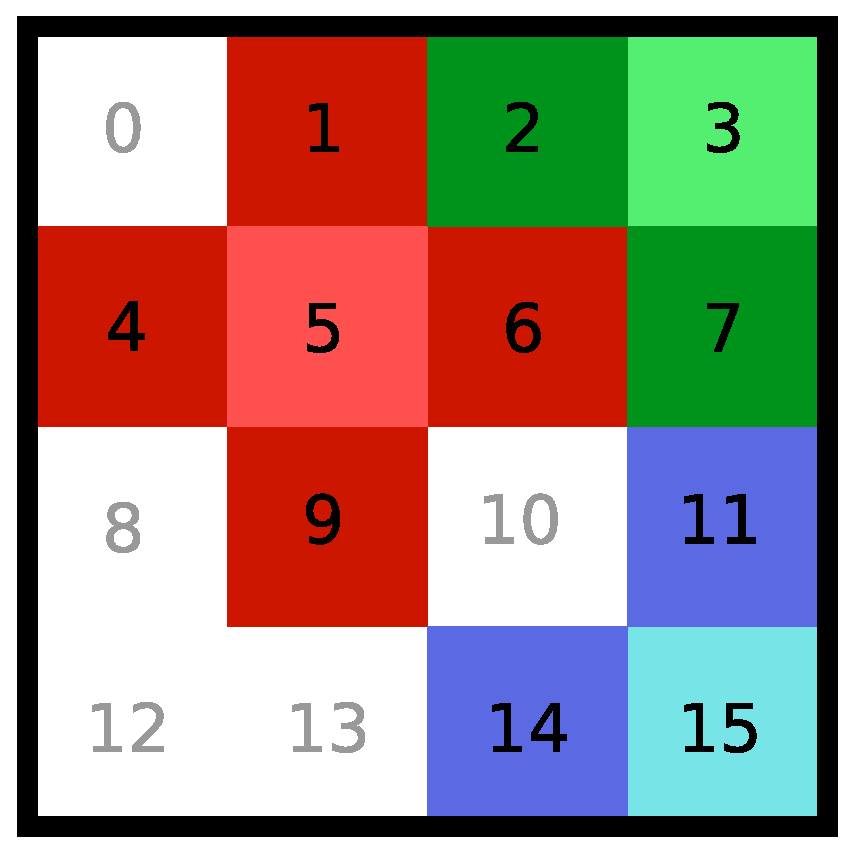
\includegraphics[width=2in]{figures/disjoint-scopes6}
    \end{center}
  }

\end{slide}

\begin{slide}{DynPSDD}
  \vspace{.2in}
  \begin{center}
    Dynamic Parallel Structured Duplicate Detection
  \end{center}

  \onslide*{1}{
  \begin{itemize}
  \item Obtains a suboptimal solution using weighted A*
  \item Uses breadth first heuristic search for PSDD
  \item Prunes nodes based on cost of suboptimal solution
  \end{itemize}
  }
  \onslide*{2}{
  \begin{center}
    What weight to use? \\
    %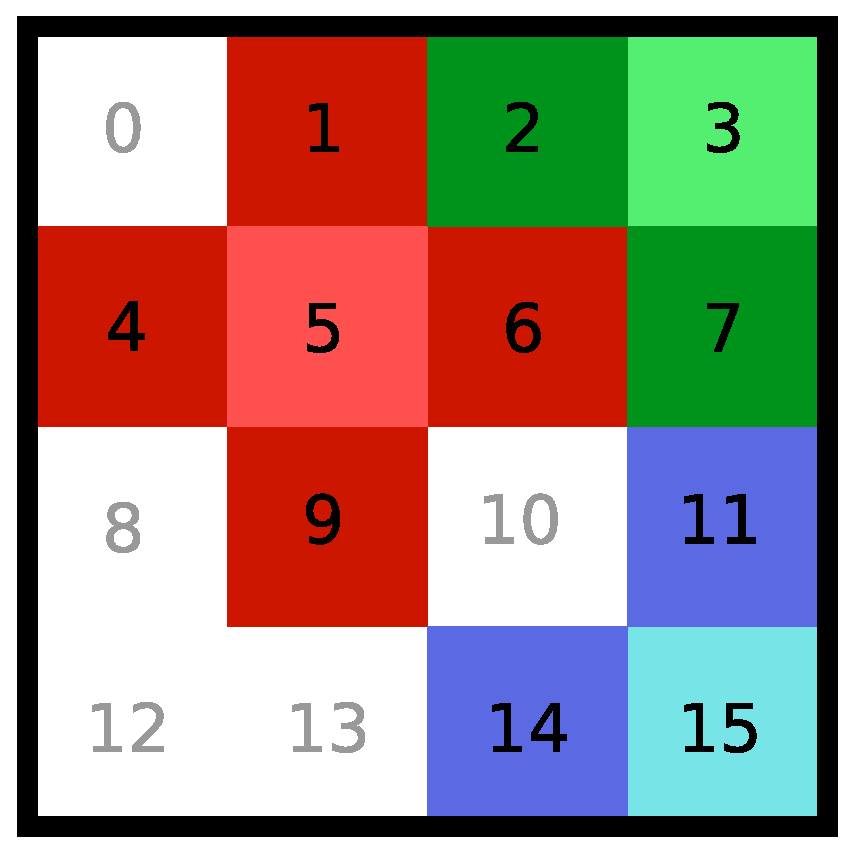
\includegraphics[width=2in]{figures/disjoint-scopes6}
  \end{center}
  }
  \onslide*{3}{
  \begin{center}
    Nblocks per thread \\
    %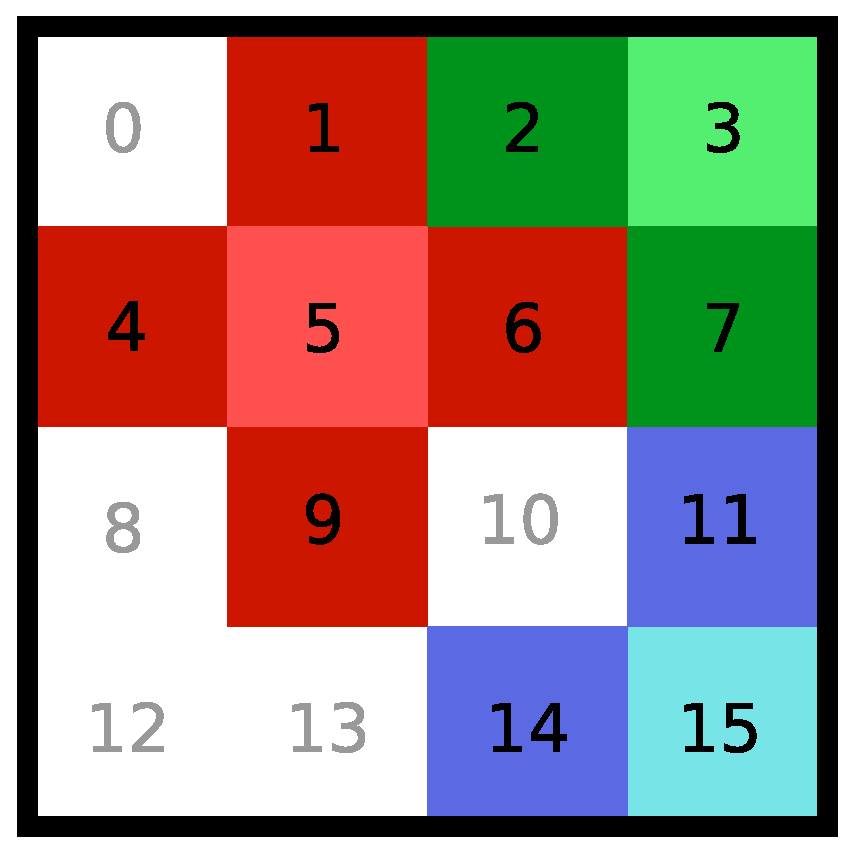
\includegraphics[width=2in]{figures/disjoint-scopes6}
  \end{center}
  }
\end{slide}

\begin{slide}{BFPSDD}
  \vspace{.2in}
  \begin{center}
    Best-First Parallel Structured Duplicate Detection
  \end{center}

  \onslide*{1}{
  \begin{itemize}
  \item Layers based on $f$ values, rather than $g$
  \item Expands fewer nodes than pure breadth first
  \end{itemize}
  }
  \onslide*{2}{
  \begin{center}
    Nblocks per thread \\
    %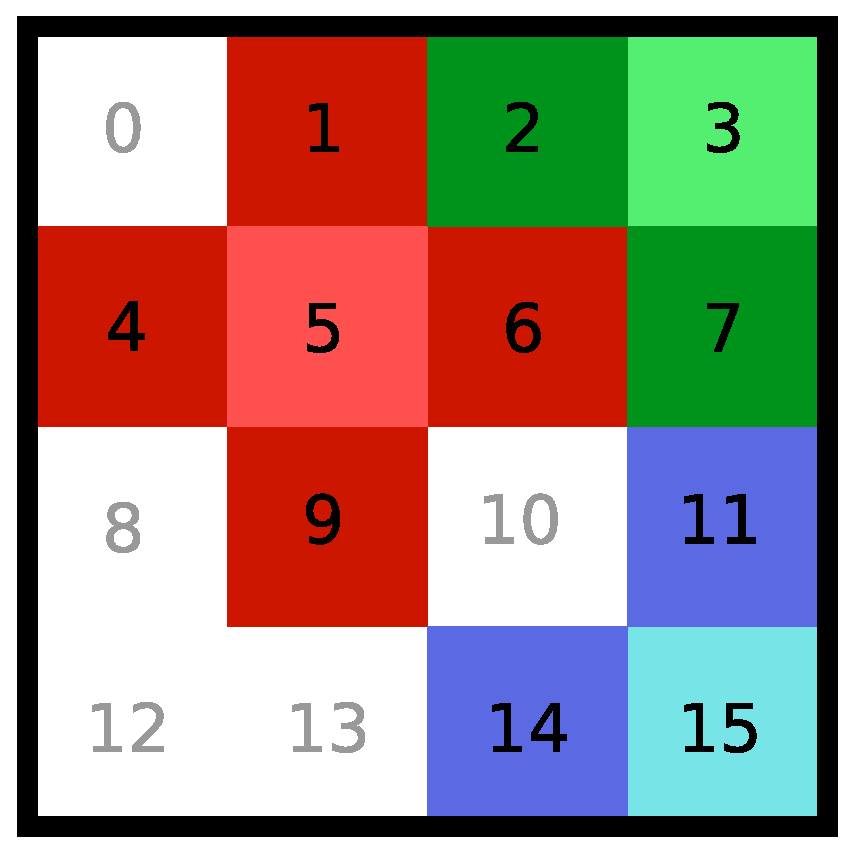
\includegraphics[width=2in]{figures/disjoint-scopes6}
  \end{center}
  }
\end{slide}

% ------------------------------------------------------------

\begin{slide}{PBNF}
  \vspace{.2in}
  \begin{center}
    Parallel Best NBlock First
  \end{center}

  \begin{itemize}
  \item Heap of free nblocks $H = \langle N_0, N_1, ..., N_n \rangle$
  \item Processors acquire the best disjoint nblocks
  \item NBlock, $N_0$, expanded while
    \begin{eqnarray*}
      (\mathop{\rm min}_{n \in N_0} f(n)) < (\mathop{\rm min}_{m \in N_{next}} f(m))
    \end{eqnarray*}
    where $N_{next}$ is the next best nblock on $H$
  \item Minimum expansions, $m$ to reduce contention
  \item No layer based synchronization
  \end{itemize}

\end{slide}

% --------------------

\begin{slide}{Safe PBNF}
  \vspace{.2in}
  \begin{center}
    Safe Parallel Best NBlock First
  \end{center}
  \onslide*{1}{
    \begin{center}
      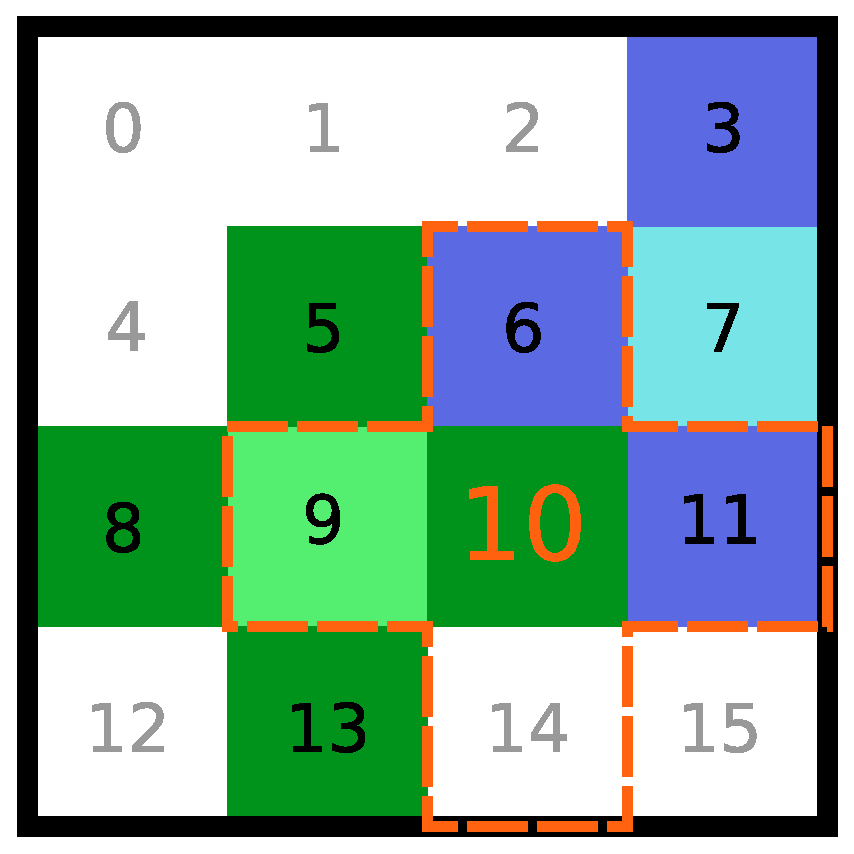
\includegraphics[width=2in]{figures/livelock0} \\
    \end{center}
  }
  \onslide*{2}{
    \begin{center}
      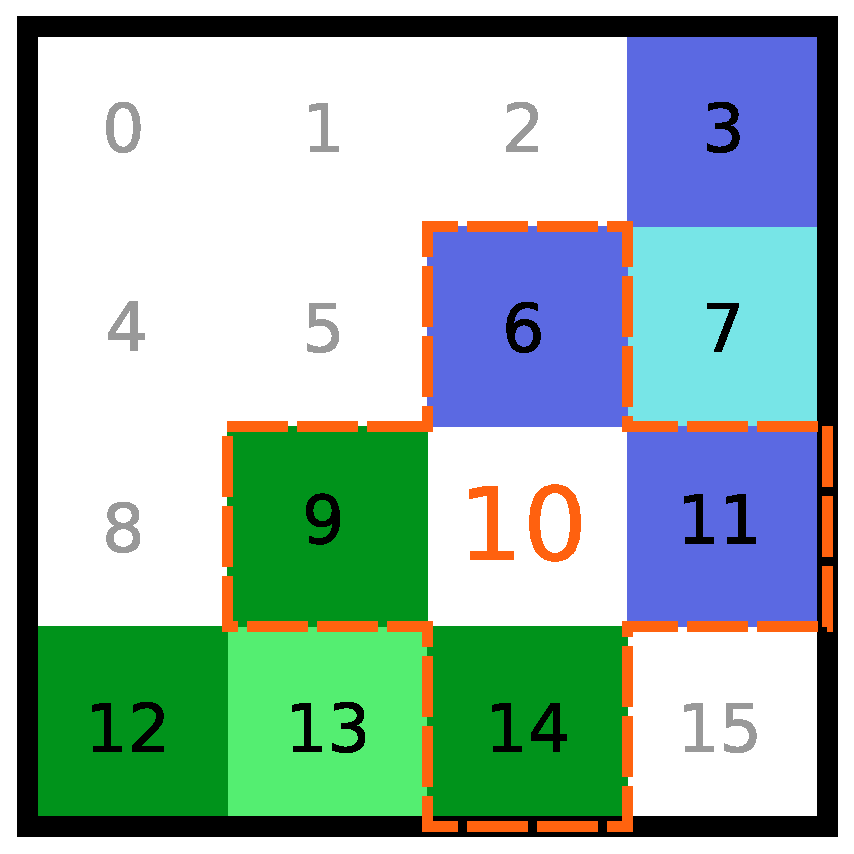
\includegraphics[width=2in]{figures/livelock1} \\
    \end{center}
  }
  \onslide*{3}{
    \begin{center}
      \includegraphics[width=2in]{figures/livelock2} \\
    \end{center}
  }
  \onslide*{4}{
    \begin{center}
      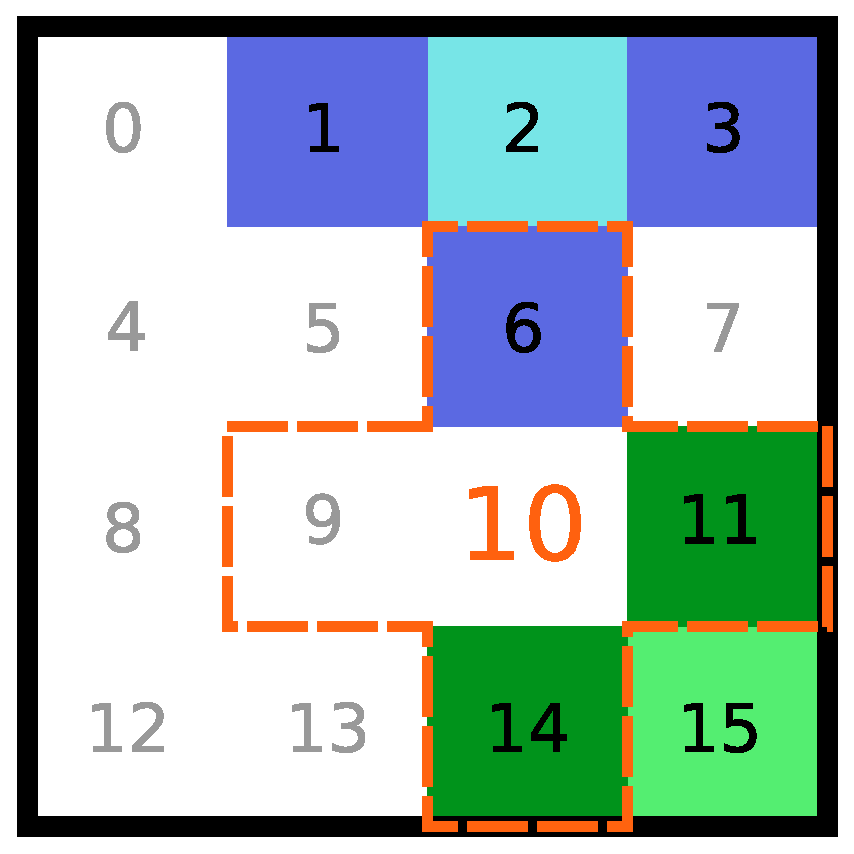
\includegraphics[width=2in]{figures/livelock3} \\
    \end{center}
  }
  \onslide*{5}{
    \begin{center}
      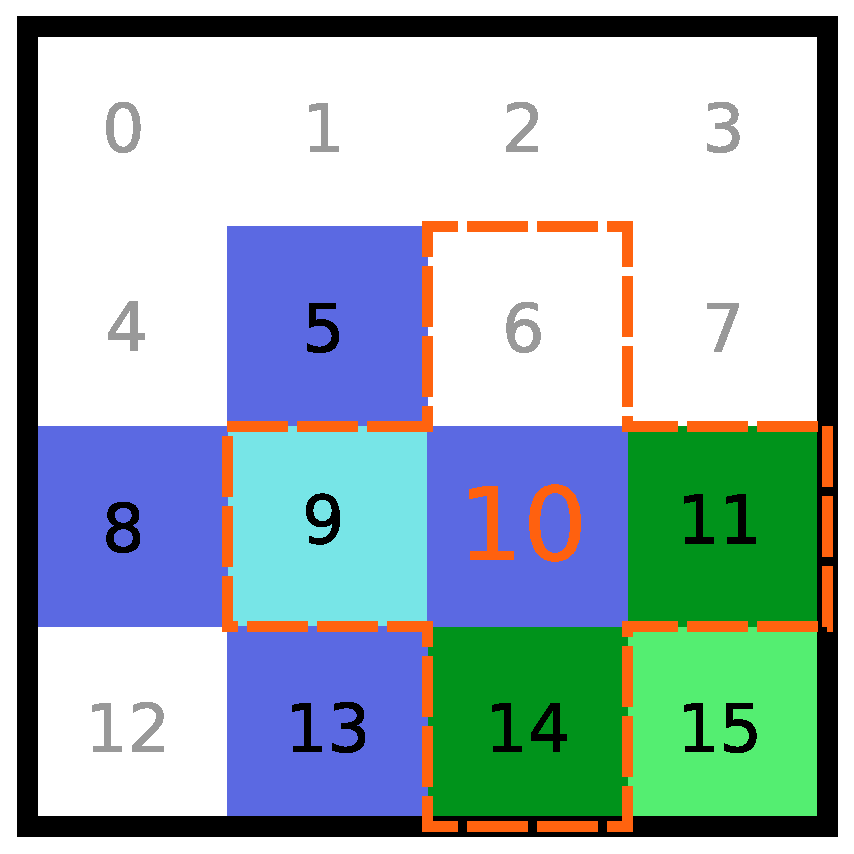
\includegraphics[width=2in]{figures/livelock4} \\
    \end{center}
  }
  \onslide*{6}{
    \begin{center}
      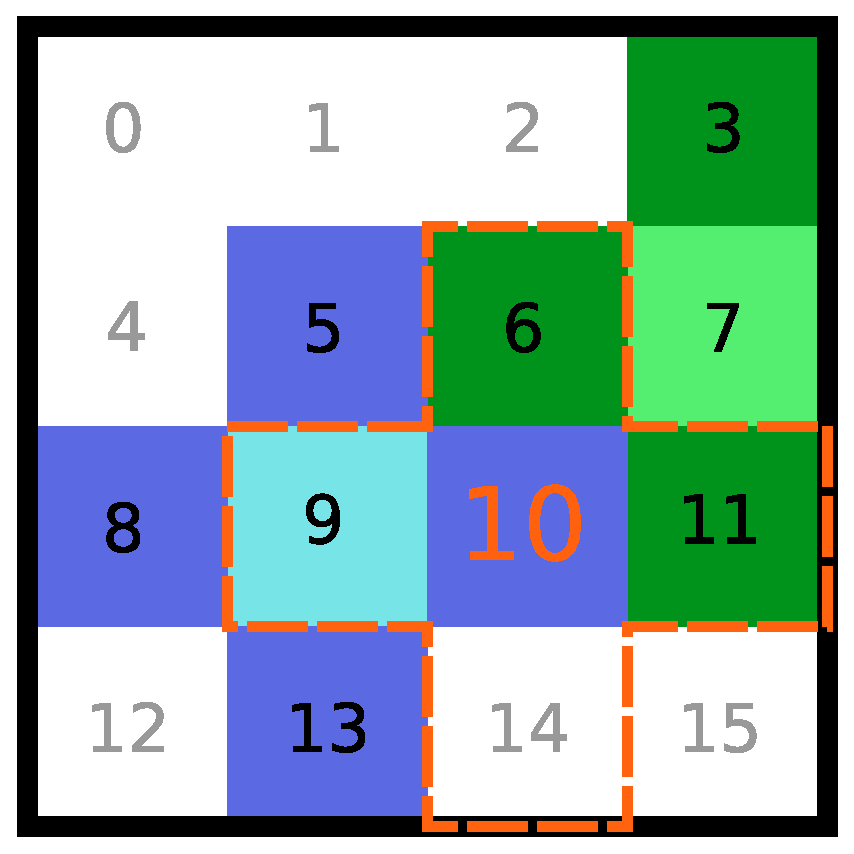
\includegraphics[width=2in]{figures/livelock5} \\
    \end{center}
  }
  \onslide*{7}{
    \begin{center}
      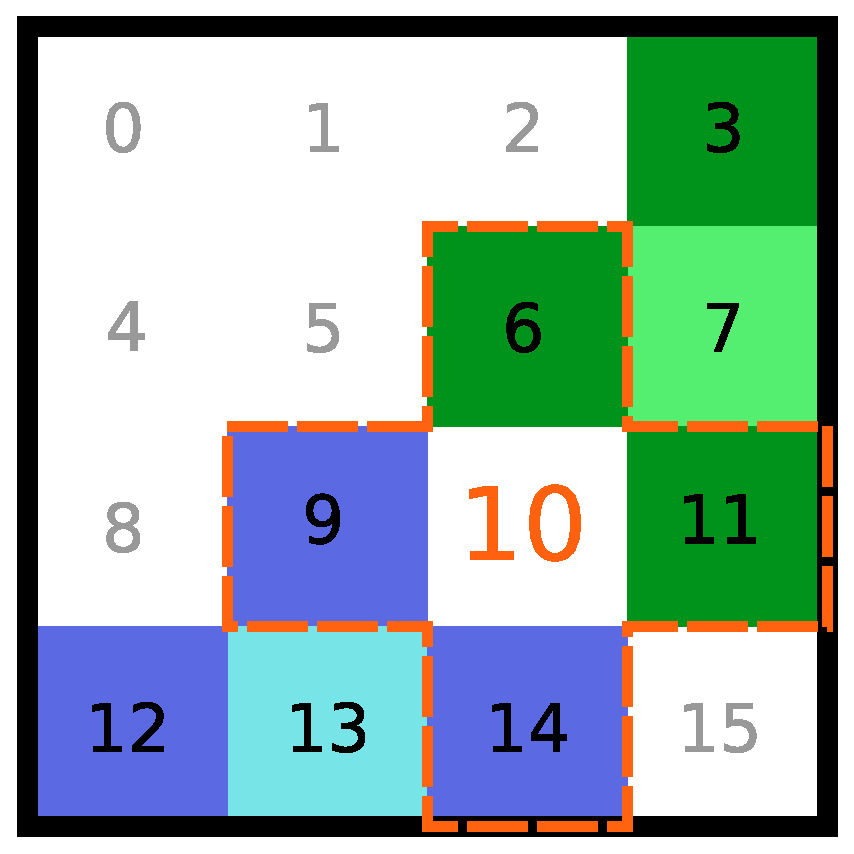
\includegraphics[width=2in]{figures/livelock6} \\
    \end{center}
  }
  \onslide*{8}{
    \begin{center}
      \includegraphics[width=2in]{figures/livelock7} \\
    \end{center}
  }
  \onslide*{9}{
    \begin{center}
      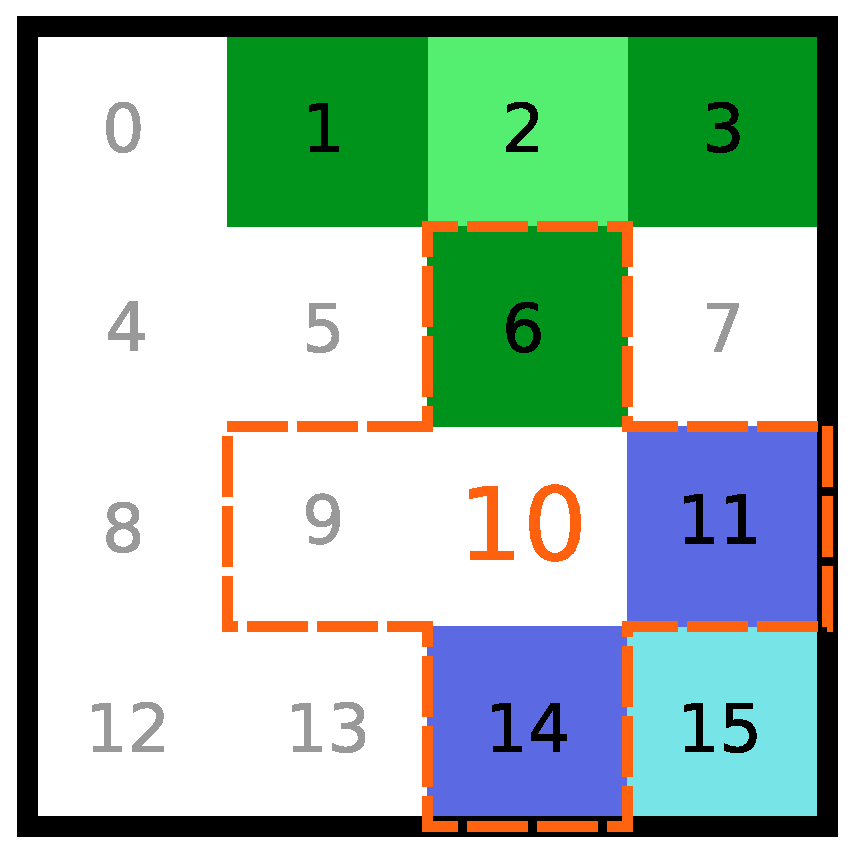
\includegraphics[width=2in]{figures/livelock8} \\
    \end{center}
  }
  \onslide*{10}{
    \begin{center}
      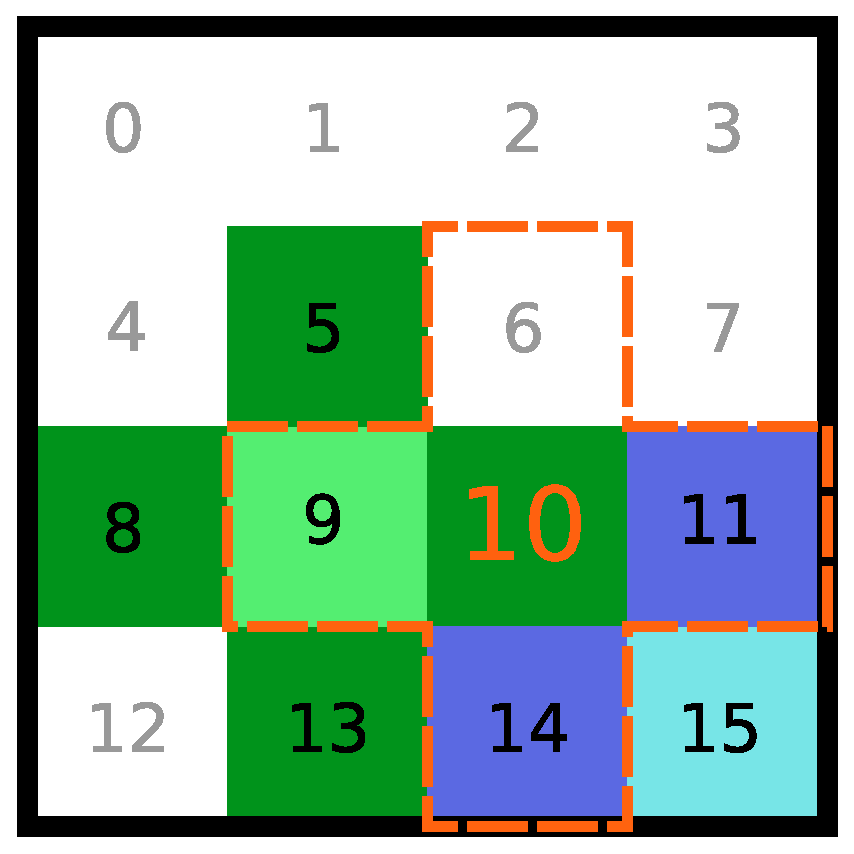
\includegraphics[width=2in]{figures/livelock9} \\
    \end{center}
  }
  \onslide*{11}{
    \begin{center}
      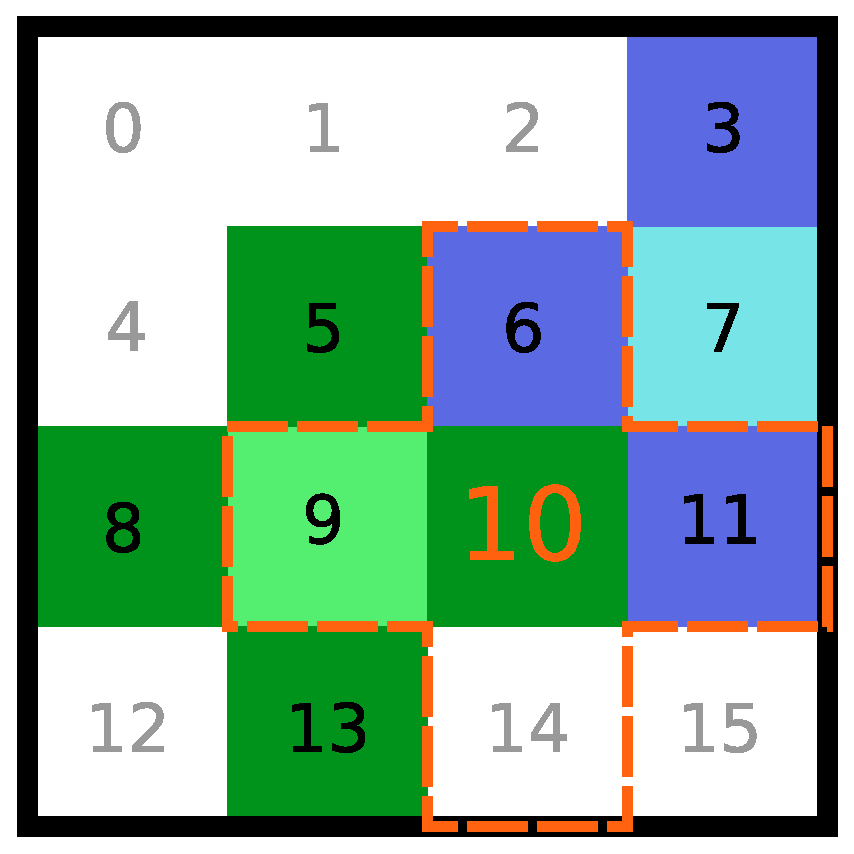
\includegraphics[width=2in]{figures/livelock0} \\
    \end{center}
  }

  \onslide*{1,2,3,4,5,6,7,8,9,10,11} {
    \vspace{-.3in}
    \begin{center}
      15-Puzzle projected on the blank
    \end{center}
  }

  \onslide*{12}{
    \begin{itemize}
    \item Mark nblocks as \emph{hot}
    \item Release nblocks which are interfering with hot nblocks
    \item Do not acquire scopes which interfere with hot nblocks
    \end{itemize}
  }
  \onslide*{13}{
    \begin{center}
      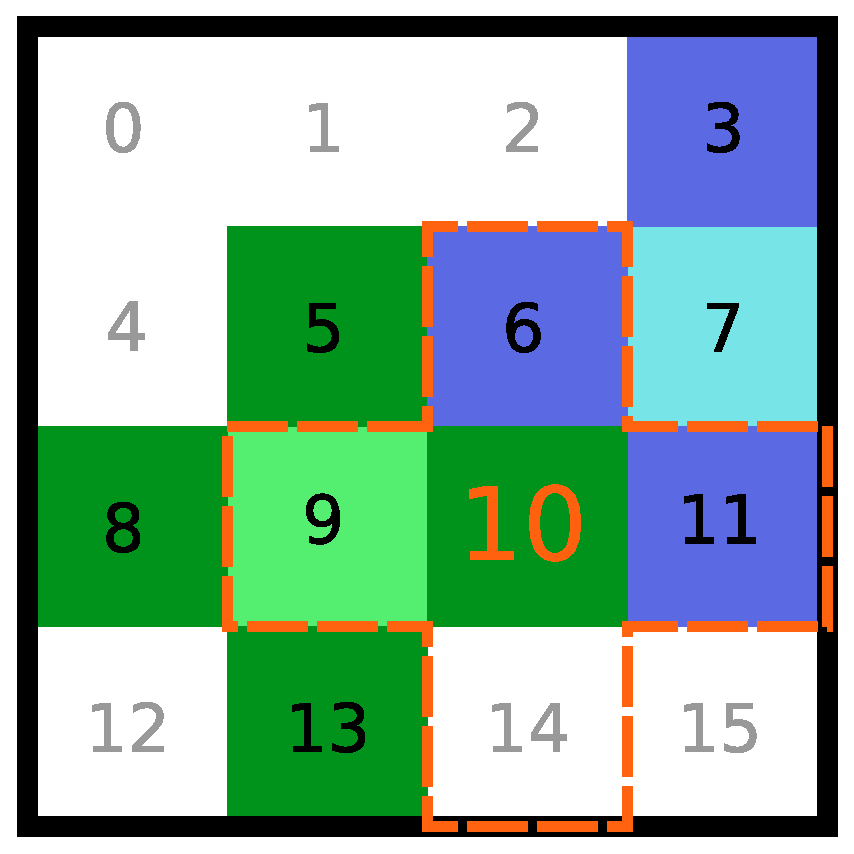
\includegraphics[width=2in]{figures/livelock0} \\
    \end{center}
  }
  \onslide*{14}{
    \begin{center}
      \includegraphics[width=2in]{figures/livelock1h} \\
    \end{center}
  }
  \onslide*{15}{
    \begin{center}
      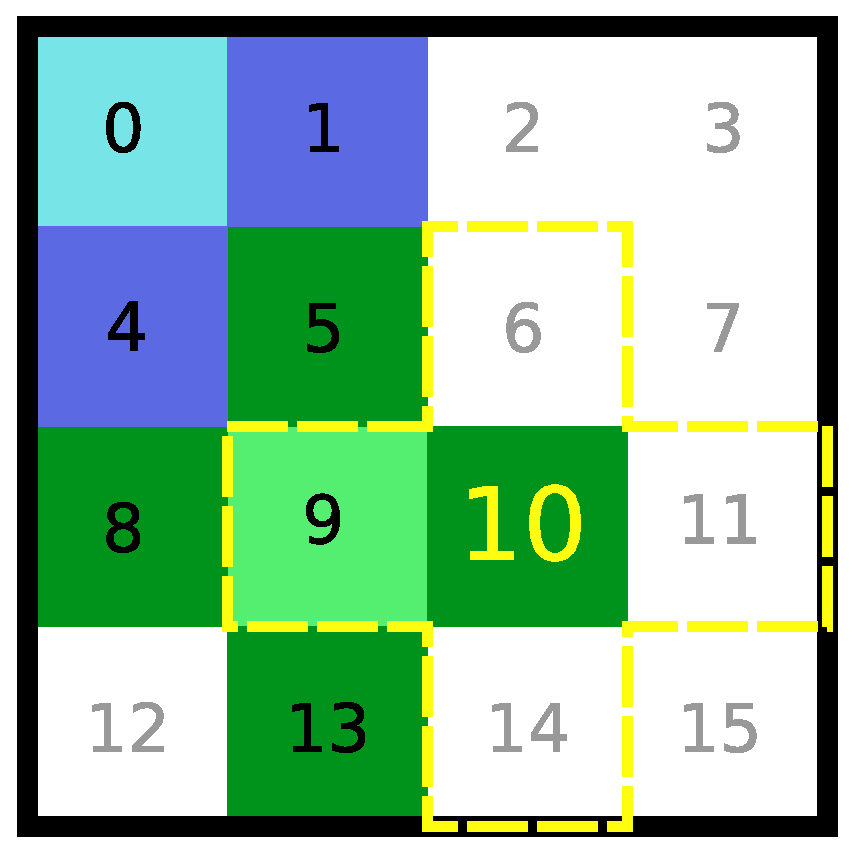
\includegraphics[width=2in]{figures/livelock2h} \\
    \end{center}
  }
  \onslide*{16}{
    \begin{center}
      \includegraphics[width=2in]{figures/livelock3h} \\
    \end{center}
  }
  \onslide*{17}{
    \begin{center}
      \includegraphics[width=2in]{figures/livelock4h} \\
    \end{center}
  }
  \onslide*{13,14,15,16,17} {
    \vspace{-.3in}
    \begin{center}
      15-Puzzle projected on the blank
    \end{center}
  }

\end{slide}

% ------------------------------------------------------------

\section{Comparison}

% --------------------

\begin{slide}{Grid World}
  \onslide*{1}{
    \begin{description}
    \item [Width] 2000
    \item [Height] 1200
    \item [Obstacle distribution] Uniform 0.25
    \item [Costs] Unit and Life
    \item [Start] Bottom Left
    \item [Goal] Bottom Right
    \item[Projection] $(row {\rm MOD} M)$, where $M$ is a parameter
      which allows us to choose the number of nblocks and $row$ is the
      row of the grid state.
    \end{description}
  }
  \onslide*{2}{
    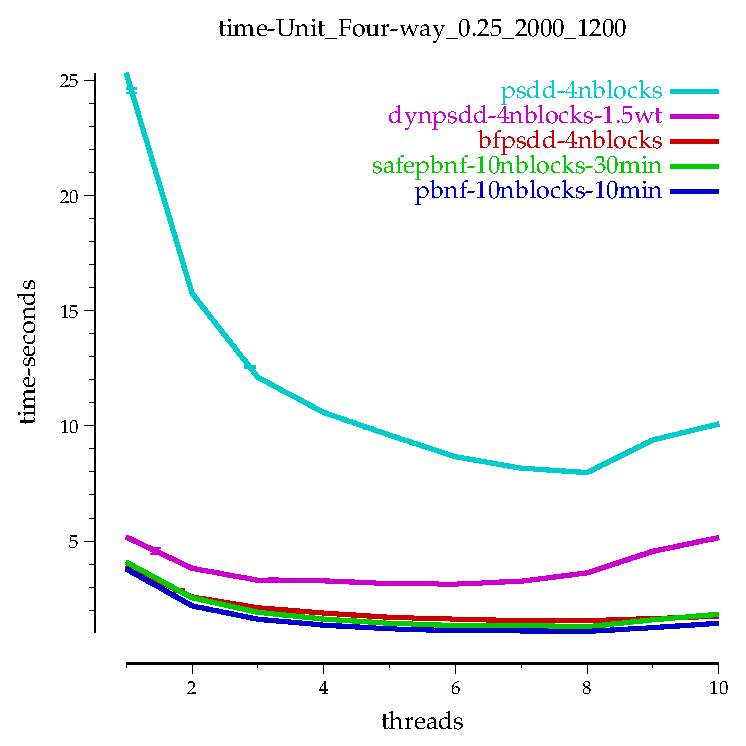
\includegraphics[width=4in,height=3in]{figures/time-Unit_Four-way_0_25_2000_1200}
  }
  \onslide*{3}{
    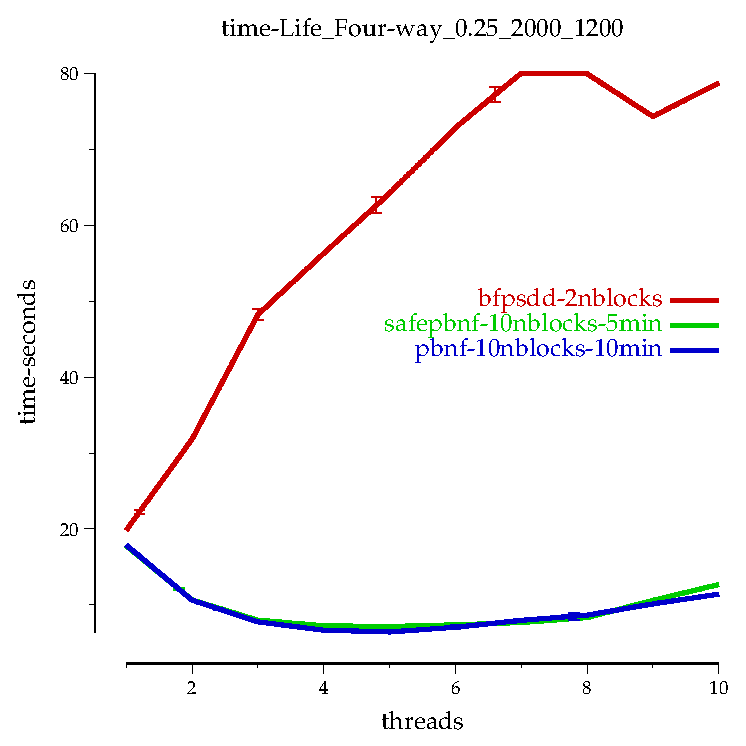
\includegraphics[width=4in,height=3in]{figures/time-Life_Four-way_0_25_2000_1200}
  }
\end{slide}

% --------------------

\begin{slide}{Sliding Tiles}
  \onslide*{1}{
    \begin{description}
    \item [Width] 7
    \item [Height] 2
    \item [Costs] Unit
    \item [Projection] The blank and the 1-tile.
    \end{description}
  }
  \onslide*{2}{
    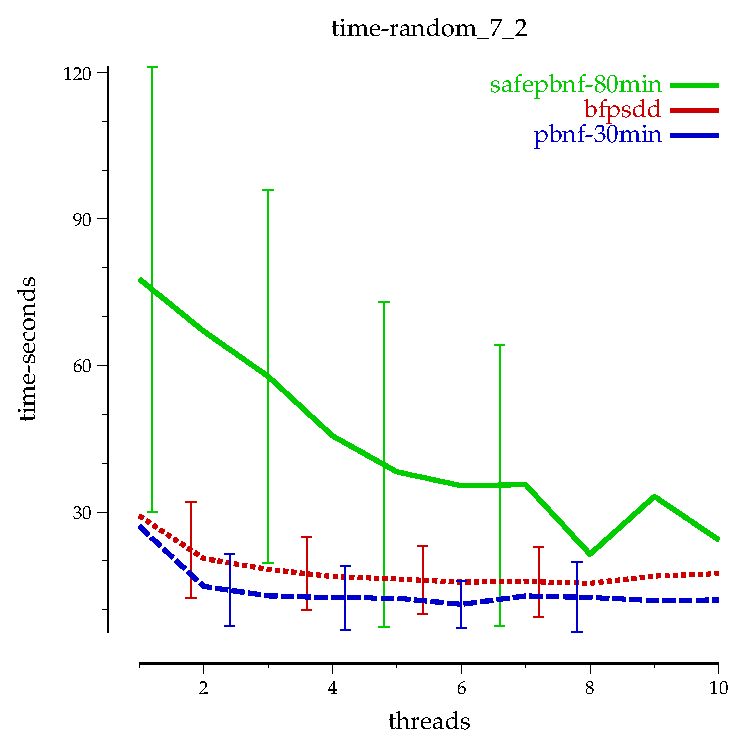
\includegraphics[width=4in,height=3in]{figures/time-random_7_2}
  }
\end{slide}

% ------------------------------------------------------------

\section{Conclusion}

% --------------------

\begin{slide}{Summary}
  \begin{center}
    Parallel Best NBlock First
  \end{center}
  \begin{itemize}
  \item Parallel best-first style search
  \item No synchronization in the ``fast-path''
  \item Performs well on a variety of domains \emph{without modification}
  \item Allows for \emph{many} possible variations:
    \begin{itemize}
    \item Weighted
    \item Pessimistic
    \item Optimistic
    \end{itemize}
  \item ``Hot Potato'' method prevents live-lock in infinite domains
  \end{itemize}
\end{slide}

% --------------------

\begin{slide}{Future Work}
  \begin{itemize}
  \item 
  \end{itemize}
\end{slide}

% --------------------

\begin{slide}{Questions}
\end{slide}{Questions}

% ------------------------------------------------------------

\end{document}
